\chapter{Secuenciador Digital de Excitación}
\label{sec:secuenciador_digital}

Para hacer girar un motor bipolar hay que invertir la corriente de sus dos bobinas en un orden cíclico. En esta
placa esa secuencia se genera por hardware sin microcontrolador local, usando dos integrados: un registro de
cuatro biestables tipo D \texttt{IC2} (\texttt{SN74LS175N}) y un multiplexor analógico doble \texttt{IC3}
(\texttt{CD4052BF}). A partir de \texttt{STEP} y \texttt{DIR}, ambos producen las cuatro salidas
\texttt{IN1}--\texttt{IN4} hacia el puente H.

\section{Estrategia de Excitación y Topologías Evaluadas}
\label{sec:estrategia_topologias}

Adoptamos excitación de paso completo con dos fases activas al mismo tiempo: ambas bobinas conducen siempre y cada
pulso \texttt{STEP} invierte la polaridad de una sola bobina por vez. Frente a energizar una fase sola por paso,
esta variante duplica la fuerza magnética disponible y aumenta el torque de avance y retención sin requerir
regulación de corriente.

En simulación (archivo \texttt{logic/ctrl\_pap.cjs}) probamos tres formas de armar esta secuencia reversible:

\begin{enumerate}
  \item Contador reversible con biestables T/D y compuertas XOR externas.
  \item Registro de desplazamiento universal \texttt{CD40194} en lazo de anillo.
  \item Máquina de estados sincrónica con dos biestables D y dos multiplexores de realimentación.
\end{enumerate}

Elegimos la tercera opción porque concentra los cuatro biestables y sus salidas negadas en un solo integrado
(\texttt{SN74LS175N}), mientras todo el cálculo del próximo estado entra en un único multiplexor doble
(\texttt{CD4052BF}), sin agregar compuertas lógicas sueltas.

\section{Arquitectura del Secuenciador y Ecuaciones de Estado}
\label{sec:arquitectura_secuenciador}

\texttt{IC2} (\texttt{SN74LS175N}) guarda el estado actual en dos bits internos ($Q_1$ y $Q_2$) y los actualiza
en cada flanco ascendente de \texttt{STEP} (\texttt{CLK}, pin 9). Su borrado asincrónico ($\sim$\texttt{CLR},
pin 1) queda fijo a \texttt{VSS} ($+5\V$), y los dos biestables sin uso (\texttt{3D} en pin 12 y \texttt{4D} en
pin 13) se atan a \texttt{GND}.

Como cada celda del \texttt{SN74LS175N} entrega tanto la salida normal como la negada, las cuatro líneas hacia
los puentes H de \texttt{IC1} se cablean directo:

\begin{itemize}
  \item $\text{IN1} = Q_1$ (pin 2 de \texttt{IC2} a pin 5 de \texttt{IC1}) e $\text{IN2} = \overline{Q_1}$ (pin 3
    de \texttt{IC2} a pin 7 de \texttt{IC1}), que invierten la fase A (\texttt{OUT1} y \texttt{OUT2}).
  \item $\text{IN3} = Q_2$ (pin 7 de \texttt{IC2} a pin 10 de \texttt{IC1}) e $\text{IN4} = \overline{Q_2}$ (pin 6
    de \texttt{IC2} a pin 12 de \texttt{IC1}), que invierten la fase B (\texttt{OUT3} y \texttt{OUT4}).
\end{itemize}

Como \texttt{IN2} siempre vale lo opuesto a \texttt{IN1}, e \texttt{IN4} lo opuesto a \texttt{IN3}, cada puente H
aplica tensión diferencial sobre su bobina en todo momento cuando \texttt{ENABLE} está activo, sin riesgo de
cortocircuitar ramas.

Por su parte, \texttt{IC3} (\texttt{CD4052BF}) lee las salidas actuales de \texttt{IC2} y prepara en sus entradas
\texttt{1D} y \texttt{2D} cuál será el próximo estado antes del siguiente pulso. Sus pines \texttt{VSS} (8),
\texttt{VEE} (7), \texttt{INH} (6), el selector \texttt{B} (9) y los canales 2 y 3 (pines 2, 4, 11 y 15) van a
\texttt{GND}, mientras \texttt{VDD} (16) toma $+5\V$ y el selector \texttt{A} (10) recibe \texttt{DIR}:

\begin{itemize}
  \item Sección \texttt{X} (salida común pin 13 al nodo \texttt{D0}, pin 4 \texttt{1D} de \texttt{IC2}): el canal
    \texttt{X0} (pin 12) recibe $\text{IN4} = \overline{Q_2}$ y el canal \texttt{X1} (pin 14) recibe
    $\text{IN3} = Q_2$.
  \item Sección \texttt{Y} (salida común pin 3 al nodo \texttt{D1}, pin 5 \texttt{2D} de \texttt{IC2}): el canal
    \texttt{Y0} (pin 1) recibe $\text{IN1} = Q_1$ y el canal \texttt{Y1} (pin 5) recibe
    $\text{IN2} = \overline{Q_1}$.
\end{itemize}

Así quedan definidas las transiciones (\ref{eq.ej3:prox_q1}) y (\ref{eq.ej3:prox_q2}), donde $Q_1^+$ y $Q_2^+$
indican el estado tras el pulso de \texttt{STEP}:

\begin{equation}
  D_0 = Q_1^+ = \overline{\text{DIR}} \cdot \overline{Q_2} + \text{DIR} \cdot Q_2
  \label{eq.ej3:prox_q1}
\end{equation}

\begin{equation}
  D_1 = Q_2^+ = \overline{\text{DIR}} \cdot Q_1 + \text{DIR} \cdot \overline{Q_1}
  \label{eq.ej3:prox_q2}
\end{equation}

\section{Secuencia de Conmutación y Acoplamiento CMOS--TTL}
\label{sec:secuencia_acoplamiento}

Según (\ref{eq.ej3:prox_q1}) y (\ref{eq.ej3:prox_q2}), cada pulso cambia un único bit ($Q_1$ o $Q_2$),
recorriendo un código Gray de 2 bits. Con $\text{DIR} = 0$ avanza en el orden $S_0 \to S_1 \to S_2 \to S_3 \to S_0$,
y con $\text{DIR} = 1$ retrocede por el ciclo inverso. En la tabla~\ref{tab.ej3:secuencia_gray} se resumen los
cuatro estados y sus salidas.

\begin{table}[!ht]
  \centering
  \resizebox{\textwidth}{!}{
    \begin{tabular}{|c|c|c|c|c|c|c|c|c|}
      \hline
      \textbf{Estado} & $(Q_1, Q_2)$ & \textbf{IN1} & \textbf{IN2} & \textbf{IN3} & \textbf{IN4}
      & \textbf{Fases} & \textbf{Próx.} ($\text{DIR}=0$) & \textbf{Próx.} ($\text{DIR}=1$) \\ \hline
      $S_0$ & $(1, 0)$ & 1 & 0 & 0 & 1 & $A^+,\ B^-$ & $S_1: (1, 1)$ & $S_3: (0, 0)$ \\ \hline
      $S_1$ & $(1, 1)$ & 1 & 0 & 1 & 0 & $A^+,\ B^+$ & $S_2: (0, 1)$ & $S_0: (1, 0)$ \\ \hline
      $S_2$ & $(0, 1)$ & 0 & 1 & 1 & 0 & $A^-,\ B^+$ & $S_3: (0, 0)$ & $S_1: (1, 1)$ \\ \hline
      $S_3$ & $(0, 0)$ & 0 & 1 & 0 & 1 & $A^-,\ B^-$ & $S_0: (1, 0)$ & $S_2: (0, 1)$ \\ \hline
    \end{tabular}
  }
  \caption{Tabla de estados del secuenciador digital y polaridad de las fases para ambos sentidos de giro.}
  \label{tab.ej3:secuencia_gray}
\end{table}

El diagrama de la figura~\ref{fig.ej3:fsm_pasos} muestra todas las transiciones posibles, y la
figura~\ref{fig.ej3:cronograma_pasos} grafica las señales $Q_1$ y $Q_2$ desfasadas $90^\circ$ eléctricos durante
cuatro pasos de avance y cuatro de retroceso tras cambiar \texttt{DIR}.

\begin{figure}[!ht]
  \centering
  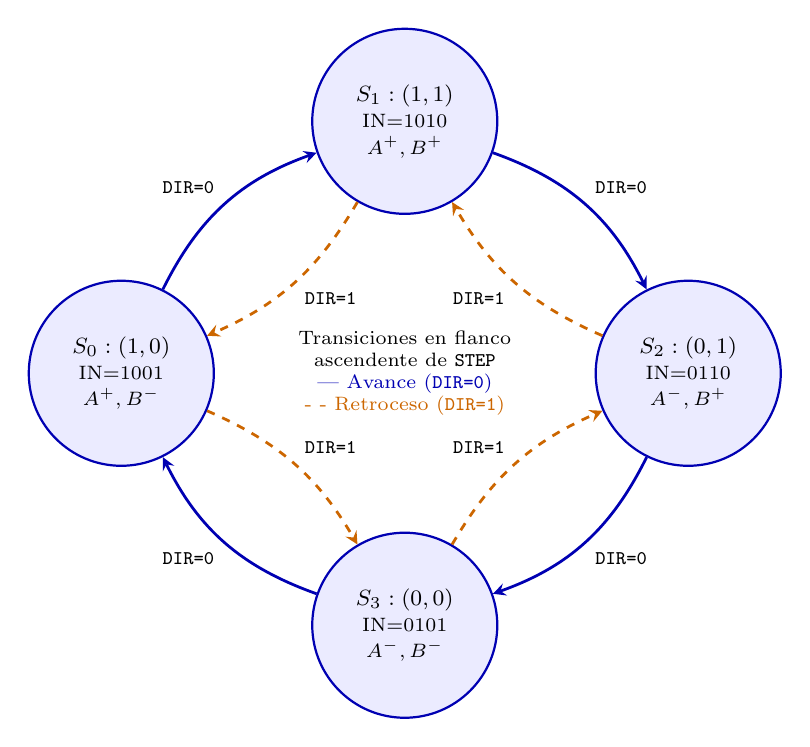
\begin{tikzpicture}[
  >=stealth, thick,
  state/.style={
    draw=blue!70!black, fill=blue!8, circle, minimum size=2.35cm, align=center, font=\footnotesize
  },
  fwd/.style={->, draw=blue!70!black, line width=1pt},
  rev/.style={->, draw=orange!80!black, line width=1pt, dashed}
]

  \node[state] (s0) at (-3.6,0) {\textbf{$S_0: (1,0)$}\\{\scriptsize IN=1001}\\{\scriptsize $A^+, B^-$}};
  \node[state] (s1) at (0,3.2)  {\textbf{$S_1: (1,1)$}\\{\scriptsize IN=1010}\\{\scriptsize $A^+, B^+$}};
  \node[state] (s2) at (3.6,0)  {\textbf{$S_2: (0,1)$}\\{\scriptsize IN=0110}\\{\scriptsize $A^-, B^+$}};
  \node[state] (s3) at (0,-3.2) {\textbf{$S_3: (0,0)$}\\{\scriptsize IN=0101}\\{\scriptsize $A^-, B^-$}};

  % Avance DIR = 0 (sentido horario)
  \draw[fwd] (s0) to[bend left=22] node[above left, font=\scriptsize] {\texttt{DIR=0}} (s1);
  \draw[fwd] (s1) to[bend left=22] node[above right, font=\scriptsize] {\texttt{DIR=0}} (s2);
  \draw[fwd] (s2) to[bend left=22] node[below right, font=\scriptsize] {\texttt{DIR=0}} (s3);
  \draw[fwd] (s3) to[bend left=22] node[below left, font=\scriptsize] {\texttt{DIR=0}} (s0);

  % Retroceso DIR = 1 (sentido antihorario)
  \draw[rev] (s1) to[bend left=18] node[below right, font=\scriptsize] {\texttt{DIR=1}} (s0);
  \draw[rev] (s2) to[bend left=18] node[below left, font=\scriptsize] {\texttt{DIR=1}} (s1);
  \draw[rev] (s3) to[bend left=18] node[above left, font=\scriptsize] {\texttt{DIR=1}} (s2);
  \draw[rev] (s0) to[bend left=18] node[above right, font=\scriptsize] {\texttt{DIR=1}} (s3);

  % Leyenda central
  \node[align=center, font=\scriptsize] at (0,0) {
    Transiciones en flanco\\ascendente de \texttt{STEP}\\
    {\color{blue!70!black}--- Avance (\texttt{DIR=0})}\\
    {\color{orange!80!black}- - Retroceso (\texttt{DIR=1})}
  };
\end{tikzpicture}

  \caption{Diagrama de transiciones de estado del secuenciador para $\text{DIR}=0$ y $\text{DIR}=1$.}
  \label{fig.ej3:fsm_pasos}
\end{figure}

\begin{figure}[!ht]
  \centering
  \resizebox{\textwidth}{!}{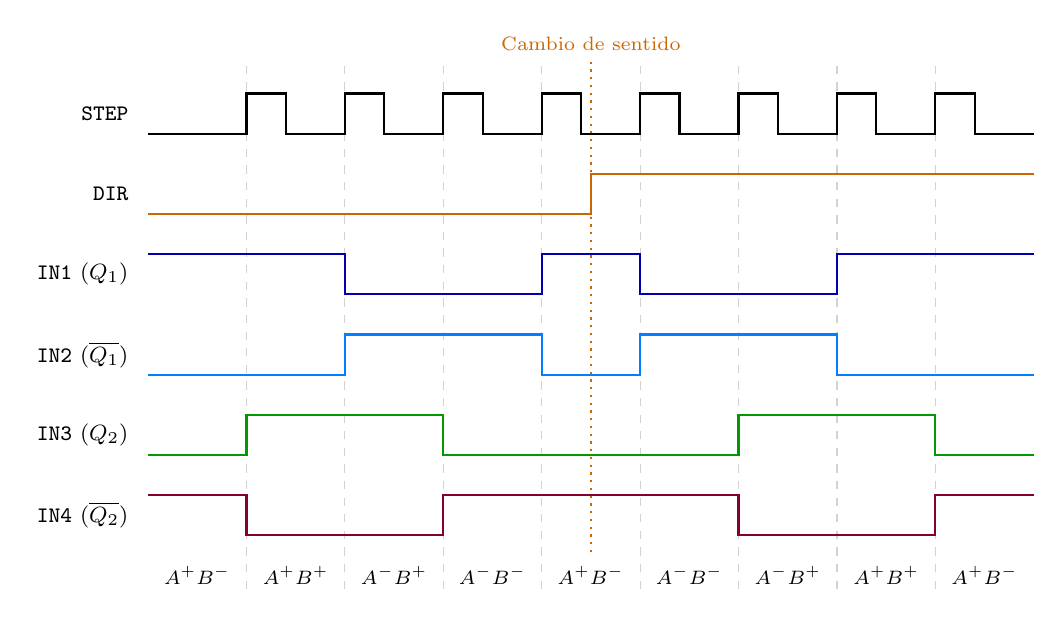
\begin{tikzpicture}[x=1.25cm, y=0.85cm, font=\footnotesize]
  % Grilla vertical de referencia en cada flanco ascendente de STEP
  \foreach \x in {1,2,3,4,5,6,7,8} {
    \draw[gray!35, dashed] (\x, -0.3) -- (\x, 7.6);
  }
  % Linea de cambio de DIR (termina sobre las etiquetas de estado)
  \draw[orange!80!black, dotted, thick] (4.5, 0.25) -- (4.5, 7.6);

  % Etiquetas de canales a la izquierda
  \node[left] at (-0.1, 6.8) {\texttt{STEP}};
  \node[left] at (-0.1, 5.6) {\texttt{DIR}};
  \node[left] at (-0.1, 4.4) {\texttt{IN1} ($Q_1$)};
  \node[left] at (-0.1, 3.2) {\texttt{IN2} ($\overline{Q_1}$)};
  \node[left] at (-0.1, 2.0) {\texttt{IN3} ($Q_2$)};
  \node[left] at (-0.1, 0.8) {\texttt{IN4} ($\overline{Q_2}$)};

  % STEP (pulsos en t = 1..8)
  \draw[thick, black]
    (0,6.5) -- (1,6.5) -- (1,7.1) -- (1.4,7.1) -- (1.4,6.5) --
    (2,6.5) -- (2,7.1) -- (2.4,7.1) -- (2.4,6.5) --
    (3,6.5) -- (3,7.1) -- (3.4,7.1) -- (3.4,6.5) --
    (4,6.5) -- (4,7.1) -- (4.4,7.1) -- (4.4,6.5) --
    (5,6.5) -- (5,7.1) -- (5.4,7.1) -- (5.4,6.5) --
    (6,6.5) -- (6,7.1) -- (6.4,7.1) -- (6.4,6.5) --
    (7,6.5) -- (7,7.1) -- (7.4,7.1) -- (7.4,6.5) --
    (8,6.5) -- (8,7.1) -- (8.4,7.1) -- (8.4,6.5) -- (9,6.5);

  % DIR (0 para t < 4.5, 1 para t >= 4.5)
  \draw[thick, orange!80!black]
    (0,5.3) -- (4.5,5.3) -- (4.5,5.9) -- (9,5.9);

  % IN1 = Q1: [0,2]=1, [2,4]=0, [4,5]=1, [5,7]=0, [7,9]=1
  \draw[thick, blue!70!black]
    (0,4.7) -- (2,4.7) -- (2,4.1) -- (4,4.1) -- (4,4.7) --
    (5,4.7) -- (5,4.1) -- (7,4.1) -- (7,4.7) -- (9,4.7);

  % IN2 = /Q1: [0,2]=0, [2,4]=1, [4,5]=0, [5,7]=1, [7,9]=0
  \draw[thick, blue!50!cyan]
    (0,2.9) -- (2,2.9) -- (2,3.5) -- (4,3.5) -- (4,2.9) --
    (5,2.9) -- (5,3.5) -- (7,3.5) -- (7,2.9) -- (9,2.9);

  % IN3 = Q2: [0,1]=0, [1,3]=1, [3,6]=0, [6,8]=1, [8,9]=0
  \draw[thick, green!60!black]
    (0,1.7) -- (1,1.7) -- (1,2.3) -- (3,2.3) -- (3,1.7) --
    (6,1.7) -- (6,2.3) -- (8,2.3) -- (8,1.7) -- (9,1.7);

  % IN4 = /Q2: [0,1]=1, [1,3]=0, [3,6]=1, [6,8]=0, [8,9]=1
  \draw[thick, purple!70!black]
    (0,1.1) -- (1,1.1) -- (1,0.5) -- (3,0.5) -- (3,1.1) --
    (6,1.1) -- (6,0.5) -- (8,0.5) -- (8,1.1) -- (9,1.1);

  % Estados resultantes por intervalo
  \node[font=\scriptsize] at (0.5, -0.1) {$A^+ B^-$};
  \node[font=\scriptsize] at (1.5, -0.1) {$A^+ B^+$};
  \node[font=\scriptsize] at (2.5, -0.1) {$A^- B^+$};
  \node[font=\scriptsize] at (3.5, -0.1) {$A^- B^-$};
  \node[font=\scriptsize] at (4.5, -0.1) {$A^+ B^-$};
  \node[font=\scriptsize] at (5.5, -0.1) {$A^- B^-$};
  \node[font=\scriptsize] at (6.5, -0.1) {$A^- B^+$};
  \node[font=\scriptsize] at (7.5, -0.1) {$A^+ B^+$};
  \node[font=\scriptsize] at (8.5, -0.1) {$A^+ B^-$};

  \node[above, font=\scriptsize, orange!80!black] at (4.5, 7.6) {Cambio de sentido};
\end{tikzpicture}
}
  \caption{Cronograma de conmutación en cuadratura ante pulsos de \texttt{STEP} e inversión de \texttt{DIR}.}
  \label{fig.ej3:cronograma_pasos}
\end{figure}

Entre la salida del multiplexor \texttt{IC3} y las entradas \texttt{1D} y \texttt{2D} de \texttt{IC2} aparecen
los resistores \texttt{R7} y \texttt{R8} ($6.8\kohm$ a \texttt{GND}). Al cambiar \texttt{DIR}, las llaves del
\texttt{CD4052BF} se abren un instante antes de cerrar el nuevo canal ($t_p \le 720\ns$) y presentan una
resistencia serie $r_{\text{ON}} \approx 470\ohm$ típica ($1050\ohm$ máx. a $25\Celsius$). Como las entradas TTL
del \texttt{SN74LS175N} entregan $I_{IL(\max)} = -0.4\mA$ y flotan hacia nivel alto si quedan sueltas,
\texttt{R7} y \texttt{R8} fijan una referencia segura a masa durante esa transición y en nivel bajo.

En nivel alto, con salida mínima de \texttt{IC2} $V_{OH(\min)} = 2.7\V$ ($3.5\V$ típico), el divisor entre
$r_{\text{ON}(\max)}$ y \texttt{R7}/\texttt{R8} entrega en la entrada de datos:

\begin{equation*}
  V_{D(\text{min})} = V_{OH(\min)} \cdot \frac{R_{7,8}}{R_{7,8} + r_{\text{ON}(\max)}}
  = 2.7\V \cdot \frac{6.8\kohm}{6.8\kohm + 1.05\kohm} \approx 2.34\V
\end{equation*}

Como supera el umbral $V_{IH(\min)} = 2.0\V$ del \texttt{SN74LS175N} incluso en el peor caso, los datos se
capturan sin errores. Los retardos combinados suman menos de $1\us$, muy por debajo de la frecuencia de trabajo
de cualquier motor CNC.
